\chapter{The O'Briens in Boston}

The O'Briens were among the almost 1.5 million Irish who sailed to the United States between 1845 and 1855.\cite{Miller:291} William\textsuperscript{1}'s two youngest children, Michael\textsuperscript{2} and Mary\textsuperscript{2}, were likely the first of the O'Brien family to make the voyage. Irish families often could only afford tickets for one or two people, and so would choose the youngest and healthiest children.\cite{Miller:292} Once in America, the children would send remittances back to Ireland until the rest of the family could be brought over.\cite{Miller:295}

\begin{figure}
	\centering
	\includegraphics[width=\textwidth]{clipper_barque}
	\caption{Example of a clipper barque from 1854. Thomas Goldsworthy Dutton, ``Clipper barque Spirit of the Age,'' Royal Museums Greenwich (\url{https://commons.wikimedia.org/wiki/File:Clipper_barque_Spirit_of_the_Age,_PY0633.jpg}).}
\end{figure}


\begin{figure}
	\centering
	\includegraphics[width=\textwidth]{mary_michael}
	\caption{Passenger list of the \textit{Thomas Baker} showing Mary O'Brien and Michael O'Brien.\cite{ThomasBaker}}
\end{figure}

\begin{figure}
	\centering
	\includegraphics[width=\textwidth]{edward_ship}
	\caption{Passenger list of the \textit{Chasca} showing O'Brien family along with ages and occupations.\cite{Chascay}}
\end{figure}

Ship passenger lists for the Port of New York show a Mary O'Brien, age 20, and Michael O'Brien, age 15, arriving on the brig \textit{Thomas Baker} from Galway, Ireland, on 3 July 1849. There were 93 total passengers aboard. The occupation listed for everyone on the passenger manifest is ``farming.''\cite{ThomasBaker}

Brigs like the \textit{Thomas Baker} were two-masted ships with square sails.\cite{OHanlon:35} Prior to the famine, these ships were outfitted for cargo rather than passengers.\cite{Laxton:9} The \textit{Thomas Baker}, for instance, was a coal-hauling ship.\cite{MorningAdvertiser} Compared to the three-masted liners, brigs were cramped for the number of passengers they carried, with poor ventilation and five-foot ceilings.\cite{OHanlon:33} The voyage from Ireland to the United States took anywhere from four to eight weeks.

A larger group of the O'Briens arrived in Boston on 27 June 1851 on board the vessel \textit{Chasca}\cite{Chascay}. The voyage from Liverpool, England, to Boston, Massachusetts, took 47 days.\cite{Chascay2} On board were Edward\textsuperscript{2} O'Brien (appearing as Edmund\cite{Edmund}), his father William, wife Bridget, sister Abby\textsuperscript{2} (O'Brien) Dooley, and Abby's two children, Margaret\textsuperscript{3} and Hanora\textsuperscript{3} (aka Hannah). There were a total of 256 passengers on board,\cite{Chascay3} which must have made the ship quite crowded. The \textit{Chasca} was a 658-ton clipper bark built in East Boston as a speedy cargo ship\cite{ChascaCard,Chascay} Like the \textit{Thomas Baker}, it was probably retrofitted to carry passengers in response to the large demand for transport to the New World during the famine years.

Both Abby's and Margaret's occupations are listed as ``Servt.'' in the passenger manifest.\cite{Chascay} About 2,000 Irish women in Boston were domestic workers in 1850. It was a popular trade for Irish immigrant women since they spoke English and didn't have many other opportunities for work available to them.\cite{Ryan:41}

William's remaining two children, John\textsuperscript{2} and Ann\textsuperscript{2}, made separate voyages from Ireland to Boston but cannot be found in passenger records. John must have arrived sometime prior to his marriage in 1853.\cite{John2OBrienCivilMarriage} Ann may not have arrived until 1870--1880 as she doesn't appear in any prior records.\cite{Census1880Edward} 

Like other Irish immigrants from this time period, William O'Brien and his children likely came to America to escape the famine and build a better life. While the family may have avoided starvation in Ireland, the first few years in Boston presented new challenges. The O'Briens lived in crowded tenement buildings, suffered devastating losses from communicable diseases, and likely faced anti-Catholic discrimination from the city's dominant class of Protestants.\cite{Ryan:61,Quinlan:58}
	
Moving frequently at first, the family lived predominantly in Boston's North End neighborhood during the 1850s and 1860s.\cite{NorthEndAddresses} In 1855, half of all residents of the North End were Irish.\cite{Todisco:29} Landlords had subdivided the North End's old mansions and warehouses into crowded tenement houses for renting to the newly-arrived immigrants.\cite{Goldfeld:102} Many of the tenements were not connected to sewage systems or had defective toilets, leading to high rates of infant mortality and diseases like smallpox, cholera, and tuberculosis.\cite{Goldfeld:103,Todisco:21,Ryan:48}

In 1834, Irish immigrants founded the first Catholic church in Boston's North End --- St.\ Mary's of the Sacred Heart, on the corner of Endicott and Cooper Streets.\cite{Todisco:26} John O'Brien married Mary Mahoney there in 1853.\cite{John2OBrienMarriage} St.\ Mary's quickly reached capacity, and so in 1843, St. John the Baptist Church was founded in a converted pork storehouse on Moon St.\cite{Goldfeld:101,Sullivan:128} John's children Mary\textsuperscript{3} and Ellen\textsuperscript{3} were baptized there. St.\ John's, too, became crowded, which in 1862 lead to the Catholics purchasing the New North Church at the corner of Hanover and Clark Streets and re-dedicating it as St.\ Stephen's.\cite{Sullivan:128} The O'Brien family followed many other Irish in moving from St.\ John's to St.\ Stephen's when it opened. The O'Briens' baptisms and marriages took place at St.\ Stephen's at least until Margaret Dooley's marriage there in 1873.\cite{RobertFernaldMarriage}

\begin{figure}
	\centering
	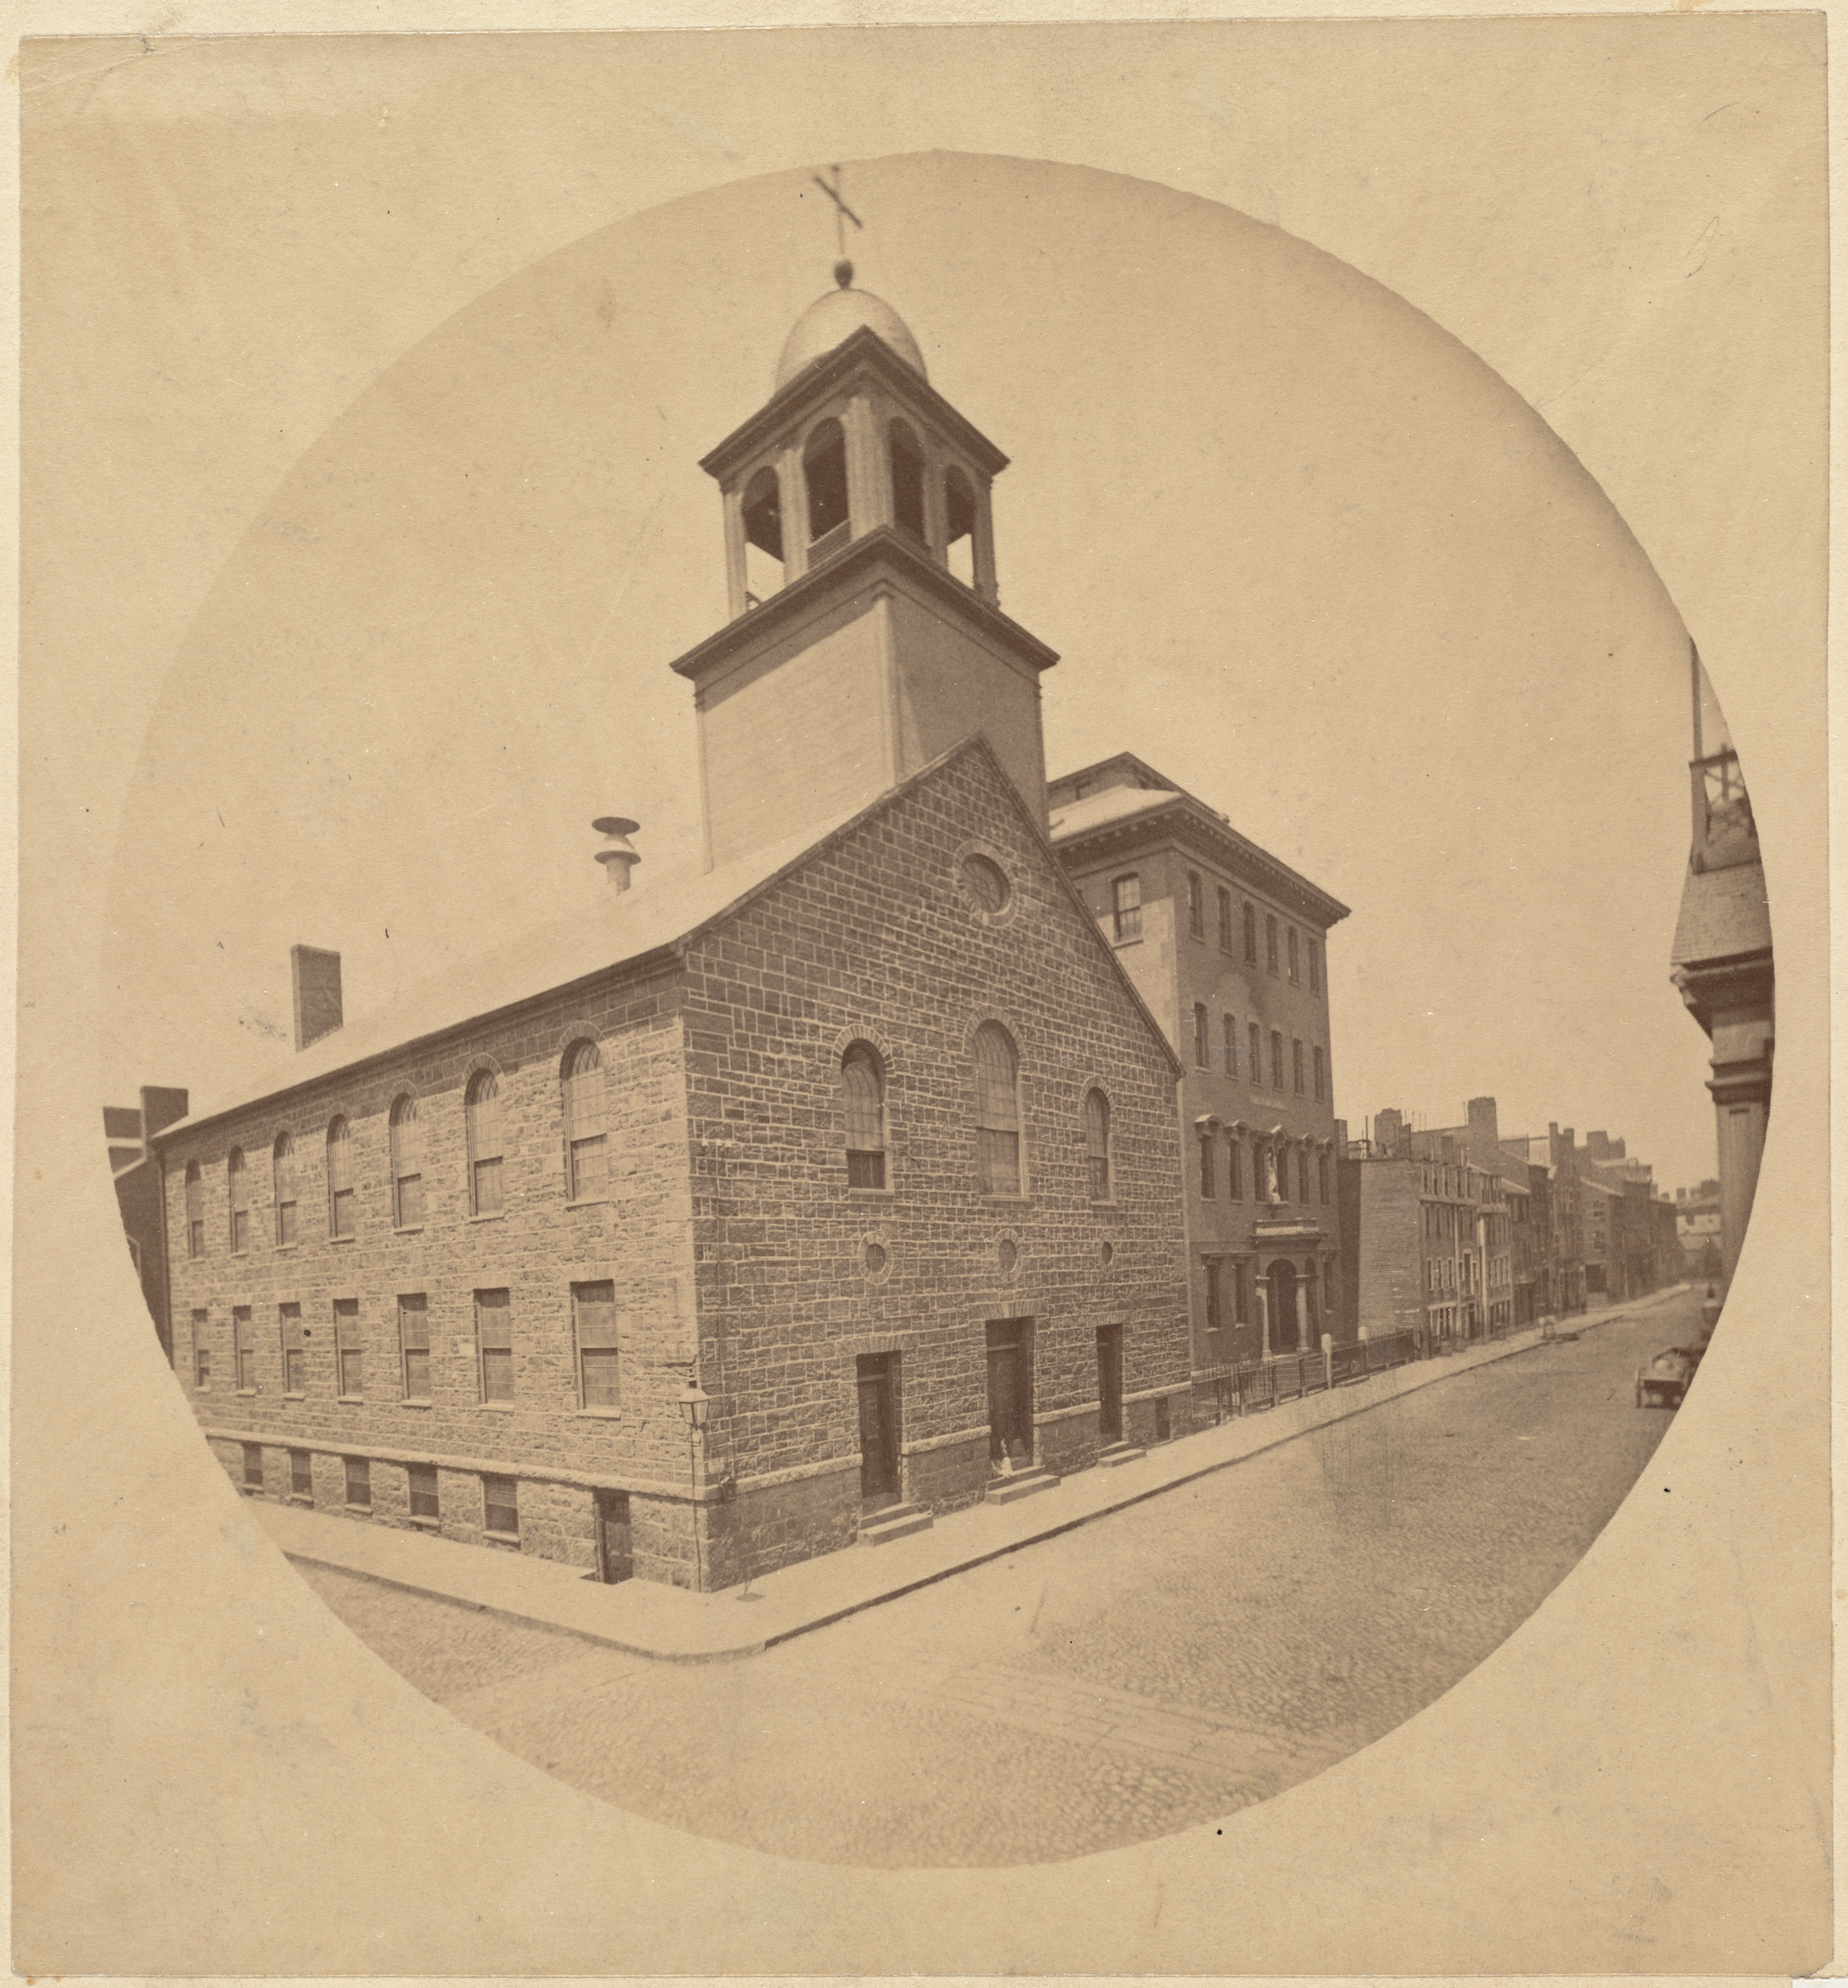
\includegraphics[width=\textwidth]{st_marys}
	\caption{Josiah Johnson Hawes, ``Old St. Mary's Church, Endicott ad Cooper Sts.,'' photograph, 1860, Boston Public Library Arts Department (\url{https://ark.digitalcommonwealth.org/ark:/50959/c821h611m}).}
\end{figure}

Irish immigrants to Boston had difficulty finding steady work, given that they were mostly rural farmers and did not have specialized trade skills.\cite{Ryan:21} Many of them started out by opening a grocery store in their tenement house or somewhere close by.\cite{Ryan:83} Indeed, John's occupation is listed as ``grocer'' on his son's birth record.\cite{John3OBrienBirth} 

John and his brother Michael both worked as oystermen.\cite{EdwardFrancis3OBrienBirth,Michael2OBrien1886,1861John2OBrien} Before the advent of industrial-scale dredging operations, the traditional method of oyster harvesting used tongs. Oyster tongs consisted of a pair of metal rakes at the end of long wooden shafts. The oysterman would use the tongs to scrape oysters off the bottom of the sea bed and manually haul them onto the boat, up to 70 pounds at a time. The boats were small vessels rigged with one or two sails.\cite{Botwick:95} Being an oysterman brought a degree of independence for an unskilled laborer. He typically owned his own boat and tackle, shucked the oysters at home to sell locally, and kept all the profits.\cite{MacKenzie:7, Botwick:96} This changed beginning in the 1870s when steam-powered oyster dredging ships arrived, and packing houses took over the oyster shucking process.\cite{MacKenzie:5, MacKenzie:7} The O'Brien brothers may have sailed to Wellfleet Harbor, Massachusetts, which had plentiful oyster beds seeded with oysters from New Haven, Connecticut.\cite{MacKenzie:29}

\begin{figure}
	\centering
	\includegraphics[width=0.3\textwidth]{oyster_tongs}
	\caption{Use of oyster tongs.\cite{MacKenzie:4}}
\end{figure}

\begin{figure}
	\centering
	\includegraphics[width=0.8\textwidth]{oyster_dredge}
	\caption{An oyster dredge at work, c.\ 1875, Popular Science Monthly Volume 6 (\url{https://commons.wikimedia.org/wiki/File:PSM_V06_D020_An_oyster_dredge_at_work.jpg}).}
\end{figure}

It seems that Edward was the main provider for the O'Brien family during the early years in Boston. He may have had a successful trade in Ireland prior to his arrival in the United States. In 1855 he was housing his father and his sister Abby's family in addition to his own.\cite{Census1855William} Edward purchased a 2-person cemetery plot at North Cambridge Catholic Cemetery in 1852\cite{CarolGordon} and a large 13-person plot at Holy Cross Cemetery in 1880\cite{HolyCrossPlot} where many of his family members were buried.

In the early 1870s, most of William's adult children (Edward, Ann, Mary, and Michael) relocated to East Boston. John's sons, John Joseph\textsuperscript{3}, Edward\textsuperscript{3}, and William\textsuperscript{3}, moved to Boston's South Cove neighborhood (now part of Chinatown).\cite{1870sAddresses} 

John's family was hit particularly hard by tuberculosis.\footnote{The terms ``phthisis'' and ``consumption'' were used at the time to describe what is now called tuberculosis.\cite{TuberculosisHistory}} Four of his children died of the disease between 1879 and 1889, as did John himself in 1863.\cite{John2OBrienDeath} In fact, John's line would have ended if not for his son John Joseph. Tuberculosis disproportionately affected Irish immigrants in Boston:

\begin{quote}
	...[t]he death rate from consumption was greatest among the colored, and among the white ... it was greatest among those whose mothers were born in Ireland or who were themselves natives of Ireland, being more than 3 times the corresponding rate for those whose mothers were born in the United States, and almost double the rate for those who were themselves natives of this country.\cite{VitalStatistics}
\end{quote}

Three of Michael's sons had jobs working in Boston's gas industry. Their roles included gas meter maker, meter tester, meter reader, and foreman. The Boston Gas Company constructed a large coal gas plant at Commercial Point in 1882. The company needed to hire a large number of unskilled laborers, and many of them were Irish immigrants.\cite{Keating:11} In the early 20th century, these jobs were highly valued, as the company (later called Boston Consolidated Gas) offered employee profit-sharing plans in 1906 and a pension plan in 1919. This provided job stability and wealth for the Irish working class.\cite{Keating:20}

The profiles later in this report include details about each descendant of William O'Brien through the 4th generation.
